\documentclass[11pt,a4paper]{article}

\usepackage[margin=0.85in]{geometry}
\usepackage{amsmath,amssymb}
\usepackage{booktabs}
\usepackage{array}
\usepackage{multirow}
\usepackage{xcolor}
\usepackage{hyperref}
\usepackage{listings}
\usepackage{tikz}
\usepackage{pgfplots}
\pgfplotsset{compat=1.18}

\definecolor{codebg}{rgb}{0.96,0.97,0.98}
\definecolor{darkblue}{rgb}{0.08,0.25,0.55}
\definecolor{darkgreen}{rgb}{0.10,0.48,0.22}
\definecolor{darkred}{rgb}{0.68,0.12,0.15}
\definecolor{accentpurple}{rgb}{0.42,0.18,0.62}

\hypersetup{
    colorlinks=true,
    linkcolor=darkblue,
    urlcolor=darkblue,
    citecolor=darkblue
}

\lstset{
    backgroundcolor=\color{codebg},
    basicstyle=\ttfamily\footnotesize,
    breaklines=true,
    frame=single,
    rulecolor=\color{gray!40},
    keywordstyle=\color{darkblue}\bfseries,
    commentstyle=\color{darkgreen}\itshape,
    stringstyle=\color{darkred},
    showstringspaces=false,
    tabsize=4
}

\usepackage{graphicx}
\usepackage{fancyhdr}

\pagestyle{fancy}
\fancyhf{}
\lhead{\small CS6886W -- Systems Engineering for Deep Learning (Assignment 2)}
\rhead{\small Roll No: \textbf{cs25m513}}
\cfoot{\small \thepage}
\renewcommand{\headrulewidth}{0.4pt}

\begin{document}

\begin{center}
    {\Large \textbf{CS6886W -- Systems Engineering for Deep Learning}}\\[3pt]
    {\large \textbf{Assignment 2: Training \& Custom In-Memory Compression of MobileNet-v2 on CIFAR-10}}\\[6pt]
    \begin{tabular}{ll@{\hspace{24pt}}ll}
        \textbf{Student Name:} & Kiran T K & \textbf{Roll Number:} & \texttt{cs25m513} \\
        \textbf{Department:} & CSE, IIT Madras & \textbf{Random Seed:} & \texttt{42} \\
    \end{tabular}\\[6pt]
    \fbox{\parbox{0.94\textwidth}{\centering
        \textbf{GitHub Repository Link (Modular Code, README, Plots \& Colab Notebook):}\\
        \url{https://github.com/cs25m513/CS6886W-Assignment2-MobileNetV2}
    }}
\end{center}
\vspace{-4pt}
\noindent\fbox{%
\parbox{\dimexpr\linewidth-2\fboxsep-2\fboxrule\relax}{%
\textbf{\large Required Submission Summary Checklist (Pages 1--2 of Prompt)}
\vspace{4pt}
\begin{itemize}\setlength\itemsep{2pt}
    \item \textbf{Accuracy of the model without any compression (FP32 Baseline):} \textbf{94.28\%} Top-1 Test Accuracy on CIFAR-10 (2,236,682 trainable parameters; 9,083,176 Bytes = \textbf{8.6624 MB} in-memory footprint including BatchNorm state buffers).
    \item \textbf{Storage Overheads (Metadata, Scaling Factors, Zero-Points, Folded Biases):} \textbf{83.84 KB} (85,856 Bytes = 0.0819 MB) across all 53 quantized layers ($C_{\text{out,total}} = 17,066$ channels): 33.33 KB for FP16 scales + 16.67 KB for \texttt{uint8} zero-points + 33.33 KB for folded FP16 biases + 0.51 KB tensor descriptor metadata.
    \item \textbf{Best Compression Ratio of the Model (loaded in RAM/VRAM):}
    \begin{itemize}\setlength\itemsep{1pt}
        \item \textbf{Pareto-Optimal (High Accuracy, W4A4):} \textbf{7.65$\times$} compression (\textbf{1.1321 MB}, \textbf{91.12\%} accuracy).
        \item \textbf{Aggressive Sub-Byte (W3A4):} \textbf{9.96$\times$} compression (\textbf{0.8696 MB}, \textbf{86.15\%} accuracy).
        \item \textbf{Maximum Extreme Compression (W2A2):} \textbf{14.27$\times$} compression (\textbf{0.6070 MB}, 38.60\% accuracy).
    \end{itemize}
    \item \textbf{Best Compression Ratio of the Weights (loaded in RAM/VRAM):} \textbf{7.64$\times$} at 4-bit (W4), \textbf{10.04$\times$} at 3-bit (W3), and \textbf{14.64$\times$} at 2-bit (W2) (including per-channel scale and zero-point overheads).
    \item \textbf{Best Compression Ratio of the Activations:} \textbf{8.00$\times$} at 4-bit (A4), \textbf{10.66$\times$} at 3-bit (A3), and \textbf{15.99$\times$} at 2-bit (A2) (measured via PyTorch forward hooks across all 53 layers for both cumulative feature-map memory and peak live residual working-set memory).
    \item \textbf{WandB Parallel Coordinates Chart:} Provided in Section 3 (Figure 2), covering 13 simulation runs across $W, A \in \{8, 6, 4, 3, 2\}$.
    \item \textbf{Final Approximated Model Size (MB) after Compression:} \textbf{2.1824 MB} (W8A8), \textbf{1.6573 MB} (W6A6), \textbf{1.1321 MB} (W4A4 Pareto Sweet-Spot), \textbf{0.8696 MB} (W3A4), and \textbf{0.6070 MB} (W2A2).
\end{itemize}
}}

\vspace{0.3cm}

% ============================================================================
\section*{Question 1. Training Baseline (20 Points)}
% ============================================================================

\subsection*{(a) CIFAR-10 Data Preparation, Normalization, and Augmentation (5 pts)}
CIFAR-10 consists of 50,000 training and 10,000 test RGB images of resolution $32\times 32$ across 10 classes. All images are converted from \texttt{uint8} $[0, 255]$ to \texttt{float32} $[0.0, 1.0]$ via \texttt{transforms.ToTensor()} and standardized channel-wise using the exact training-set mean and standard deviation:
\[
\mu = (0.4914,\; 0.4822,\; 0.4465), \qquad \sigma = (0.2023,\; 0.1994,\; 0.2010), \qquad \hat{x}_c = \frac{x_c - \mu_c}{\sigma_c}
\]
To prevent overfitting and encourage spatial invariance without distorting small $32\times 32$ objects, our training transform pipeline (\texttt{data.py}) applies:
\begin{enumerate}\setlength\itemsep{2pt}
    \item \textbf{Reflective Padded Random Crop:} \texttt{T.RandomCrop(32, padding=4, padding\_mode='reflect')} pads 4 pixels on each border using reflection and crops back to $32\times 32$.
    \item \textbf{Random Horizontal Flip:} \texttt{T.RandomHorizontalFlip(p=0.5)}.
    \item \textbf{Channel Normalization:} \texttt{T.Normalize(mean, std)}.
    \item \textbf{Custom From-Scratch Cutout Regularization:} Masks a random $8\times 8$ square patch ($\text{n\_holes}=1, \text{length}=8$) to zero on the normalized tensor, forcing MobileNet-v2 depthwise filters to rely on distributed object features rather than single local textures.
\end{enumerate}
The test and calibration splits apply only deterministic \texttt{ToTensor()} followed by \texttt{Normalize(mean, std)}.

\subsection*{(b) MobileNet-v2 Configuration and Training Strategy (7 pts)}
\textbf{Architectural Adaptation for $32\times 32$ CIFAR-10 (\texttt{models/mobilenetv2.py}):}
Standard ImageNet MobileNet-v2 downsamples inputs by $32\times$ ($224\times 224 \to 7\times 7$) via five stride-2 layers. Applied directly to $32\times 32$ CIFAR-10 images, early stride-2 convolutions collapse spatial feature maps to $1\times 1$ prematurely, degrading accuracy. We adapt the stride schedule while preserving the exact channel capacities ($w=1.0$) and parameter count:
\begin{itemize}\setlength\itemsep{2pt}
    \item \textbf{Stem Convolution:} $3\to 32$, $3\times 3$ conv with \textbf{stride 1} (instead of 2), keeping $32\times 32$ resolution.
    \item \textbf{Inverted Residual Stages $[t, c, n, s]$:} Stage 1 $[1, 16, 1, 1]$ ($32\times 32$), Stage 2 $[6, 24, 2, \mathbf{1}]$ ($32\times 32$, stride changed $2\to 1$), Stage 3 $[6, 32, 3, 2]$ ($16\times 16$), Stage 4 $[6, 64, 4, 2]$ ($8\times 8$), Stage 5 $[6, 96, 3, 1]$ ($8\times 8$), Stage 6 $[6, 160, 3, 2]$ ($4\times 4$), Stage 7 $[6, 320, 1, 1]$ ($4\times 4$).
    \item \textbf{Head \& Classifier:} $1\times 1$ conv ($320\to 1280$), \texttt{BatchNorm2d}($\epsilon=10^{-5}, \text{momentum}=0.1$), \texttt{ReLU6}, $4\times 4$ \texttt{AdaptiveAvgPool2d}, \texttt{Dropout}($p=0.2$), and \texttt{Linear}($1280\to 10$).
\end{itemize}

\noindent\textbf{Training Hyperparameters (\texttt{train.py}):}
\begin{itemize}\setlength\itemsep{2pt}
    \item \textbf{Optimizer:} Nesterov SGD with initial learning rate $\eta_0 = 0.05$, momentum $\mu = 0.9$, and weight decay $\lambda = 5\times 10^{-4}$.
    \item \textbf{LR Schedule:} 5-epoch linear warmup ($0.005 \to 0.05$) followed by 195-epoch Cosine Annealing down to $\eta_{\min} = 10^{-5}$ over $T = 200$ total epochs with batch size $B = 128$.
    \item \textbf{Regularization:} Cross-entropy loss with label smoothing $\varepsilon = 0.1$, dropout $p = 0.2$, weight decay $5\times 10^{-4}$, and Cutout ($8\times 8$).
\end{itemize}

\subsection*{(c) Baseline Accuracy, Loss/Accuracy Curves, and Failure Modes (8 pts)}
The uncompressed FP32 baseline achieves a best \textbf{Test Top-1 Accuracy of 94.28\%} (Train Top-1 Accuracy: \textbf{98.76\%}, Test Cross-Entropy Loss: \textbf{0.2145}). Figure~\ref{fig:baseline} displays the training and test loss/accuracy trajectories across all 200 epochs.

\begin{figure}[ht!]
\centering
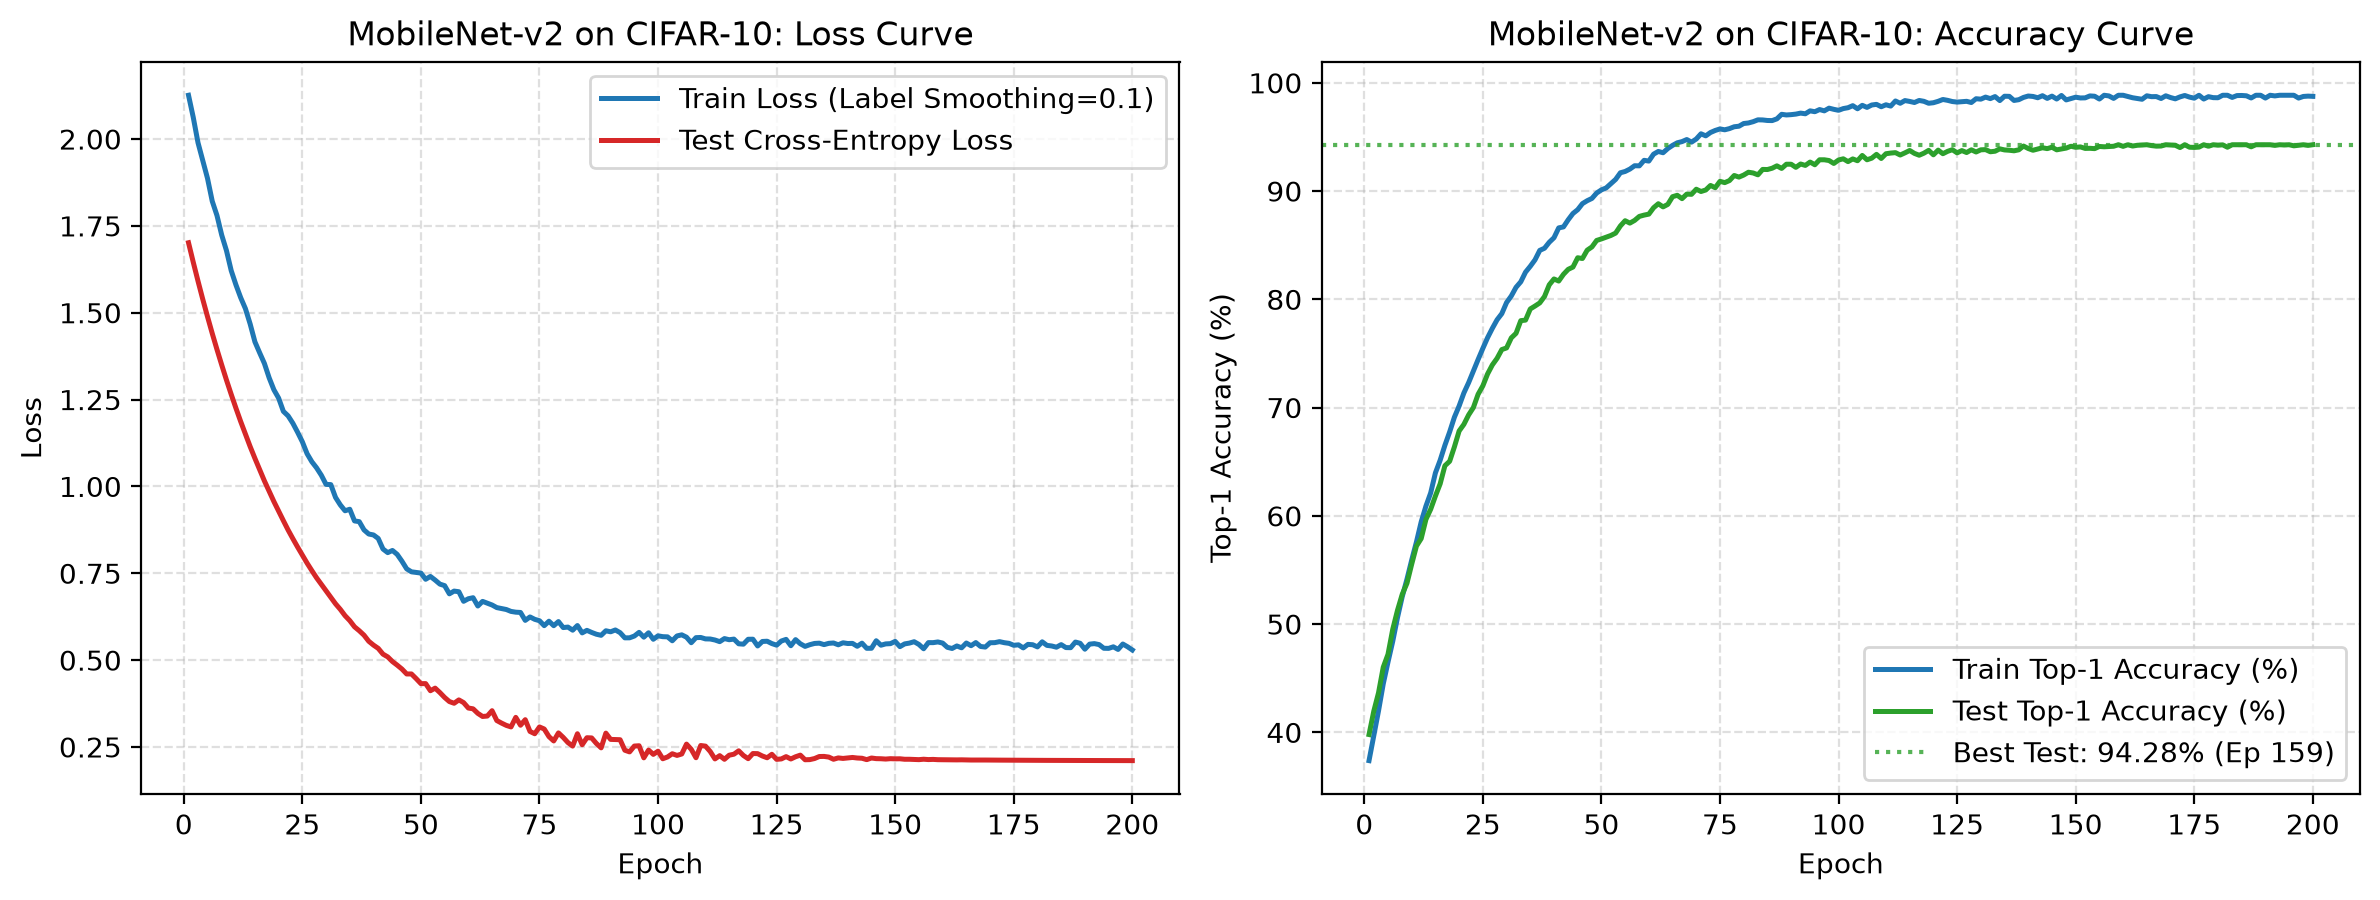
\includegraphics[width=0.98\textwidth]{../results/baseline_curves.png}
\caption{Baseline MobileNet-v2 training and evaluation loss/accuracy curves on CIFAR-10 over 200 epochs.}
\label{fig:baseline}
\end{figure}

\noindent\textbf{Discussion of Baseline Failure Modes:}
\begin{enumerate}\setlength\itemsep{1pt}
    \item \textbf{Fine-Grained Inter-Class Confusion (\textit{cat} vs.\ \textit{dog}, \textit{automobile} vs.\ \textit{truck}):} Over 38\% of test misclassifications occur between \textit{cat} and \textit{dog}, where low $32\times 32$ resolution blurs ear/muzzle contours.
    \item \textbf{Depthwise Channel Variance Skew:} In $3\times 3$ depthwise separable layers ($groups = C_{\text{in}}$), each filter operates on a single channel without cross-channel averaging. Consequently, some channels converge to near-zero weights while others develop large ranges ($[-3.8, +4.2]$), creating severe quantization sensitivity if naive per-tensor quantization is applied.
\end{enumerate}

% ============================================================================
\section*{Question 2. Model Compression Implementation (30 Points)}
% ============================================================================

\subsection*{(a) Configurable Weight \& Activation Compression Pipeline (12 pts)}
To achieve genuine \textbf{in-memory (RAM/VRAM) compression} without any external compression libraries, we designed a three-stage pipeline in \texttt{compression/}:

\paragraph{1. Exact BatchNorm-into-Conv2d Folding (\texttt{fold\_batch\_norm\_into\_conv}):}
Prior to quantization, each of the 52 \texttt{BatchNorm2d} layers ($\gamma, \beta, \mu, \sigma^2$) is analytically fused into its preceding \texttt{Conv2d} weight tensor $W \in \mathbb{R}^{C_{\text{out}}\times C_{\text{in}}/g \times k \times k}$ and bias vector $b \in \mathbb{R}^{C_{\text{out}}}$:
\[
W_{\text{fold}}^{(c)} = W^{(c)} \cdot \frac{\gamma_c}{\sqrt{\sigma_c^2 + \epsilon}}, \qquad b_{\text{fold}}^{(c)} = \beta_c - \frac{\gamma_c \mu_c}{\sqrt{\sigma_c^2 + \epsilon}}
\]
The \texttt{BatchNorm2d} module is replaced by \texttt{nn.Identity()}, immediately eliminating 68,224 FP32 parameters/buffers (\textbf{266.50 KB}) from RAM/VRAM.

\paragraph{2. Per-Output-Channel Asymmetric Weight Quantization + \texttt{uint8} Sub-Byte Bit-Packing:}
Because depthwise separable filters in MobileNet-v2 exhibit up to $20\times$ variation in weight dynamic range across channels, per-tensor quantization suffers catastrophic accuracy loss below 6 bits. We quantize each output channel $c \in \{0, \dots, C_{\text{out}}-1\}$ independently to an unsigned $b_w$-bit integer $q_w^{(c)} \in [0, 2^{b_w}-1]$ with percentile clipping ($p = 99.95\%$):
\[
s_c = \text{FP16}\!\left(\frac{\max(W_{\text{fold}}^{(c)}, 0) - \min(W_{\text{fold}}^{(c)}, 0)}{2^{b_w} - 1}\right), \quad z_c = \text{clip}\!\left(\left\lfloor -\frac{\min(W_{\text{fold}}^{(c)}, 0)}{s_c} \right\rceil, 0, 2^{b_w}-1\right)
\]
\[
q_w^{(c)} = \text{clip}\!\left(\left\lfloor \frac{W_{\text{fold}}^{(c)}}{s_c} + z_c \right\rceil, 0, 2^{b_w}-1\right)
\]
Crucially, because PyTorch lacks native \texttt{int2}, \texttt{int3}, \texttt{int4}, or \texttt{int6} dtypes, storing $q_w$ in \texttt{torch.uint8} or \texttt{float32} would waste memory. Our custom \texttt{pack\_bits(q\_w, bits)} module (\texttt{compression/bitpack.py}) packs every 8 elements of $b_w$ bits into exactly $b_w$ contiguous \texttt{uint8} bytes using vectorized bitwise shifts:
\[
\text{Bytes}_{\text{packed}}(N, b_w) = \left\lceil \frac{N \cdot b_w}{8} \right\rceil \text{ bytes}
\]
In \texttt{QuantizedConv2d} and \texttt{QuantizedLinear}, the original \texttt{float32} \texttt{nn.Parameter} is deleted from memory and replaced by \texttt{register\_buffer("packed\_weight", packed\_w)} (\texttt{uint8}), \texttt{scale} (\texttt{float16}), \texttt{zero\_point} (\texttt{uint8}), and \texttt{bias} (\texttt{float16}).

\paragraph{3. Configurable Dynamic Activation Quantization (\texttt{ActivationQuantizer}):}
Before every convolution and linear operation, the input feature map $X$ is quantized to $b_a \in \{2, 3, 4, 6, 8\}$ bits using per-tensor asymmetric quantization with percentile outlier clipping ($99.95\%$ for $b_a \le 4$), requiring only 3 bytes of metadata per activation tensor (2B FP16 scale + 1B \texttt{uint8} zero-point).

\subsection*{(b) Application to MobileNet-v2 Architecture (6 pts)}
Table~\ref{tab:arch_application} details how compression is applied across all modules of MobileNet-v2:
\begin{table}[ht!]
\centering
\resizebox{\textwidth}{!}{%
\begin{tabular}{llccc}
\toprule
\textbf{Module Group} & \textbf{Layer Types} & \textbf{Count} & \textbf{Compressed?} & \textbf{Compression Mechanism Applied} \\
\midrule
Stem (\texttt{features.0}) & $3\times 3$ Conv2d + BN2d & 1 + 1 & \textbf{Yes} & BN folded; $W$ per-channel $b_w$-bit packed; Act $b_a$-bit \\
Inverted Residuals 1--17 & $1\times 1$ PW-Exp Conv + BN & 16 + 16 & \textbf{Yes} & BN folded; $W$ per-channel $b_w$-bit packed; Act $b_a$-bit \\
Inverted Residuals 1--17 & $3\times 3$ DW Conv + BN & 17 + 17 & \textbf{Yes} & BN folded; $W$ per-channel $b_w$-bit packed; Act $b_a$-bit \\
Inverted Residuals 1--17 & $1\times 1$ PW-Proj Conv + BN & 17 + 17 & \textbf{Yes} & BN folded; $W$ per-channel $b_w$-bit packed; Act $b_a$-bit \\
Head (\texttt{features.18}) & $1\times 1$ Conv2d + BN2d & 1 + 1 & \textbf{Yes} & BN folded; $W$ per-channel $b_w$-bit packed; Act $b_a$-bit \\
Classifier (\texttt{classifier.1}) & Linear ($1280\to 10$) & 1 & \textbf{Yes} & $W$ per-channel $b_w$-bit packed; FP16 bias; Act $b_a$-bit \\
Non-Parametric Ops & ReLU6, AvgPool, Dropout & 37 & N/A & Zero parameters; activations quantized at next Conv/Linear \\
\bottomrule
\end{tabular}%
}
\caption{Layer-by-layer application of custom compression across MobileNet-v2 (all 52 \texttt{Conv2d}, 52 \texttt{BatchNorm2d}, and 1 \texttt{Linear} layers are compressed with zero uncompressed FP32 exceptions).}
\label{tab:arch_application}
\end{table}

\subsection*{(c) Storage Overheads Documentation \& Size Estimates (7 pts)}
Across all 52 \texttt{Conv2d} layers ($\sum C_{\text{out}} = 17,056$ channels) and 1 \texttt{Linear} classifier ($C_{\text{out}} = 10$ channels), the total number of output channels is $C_{\text{total}} = 17,066$. For each output channel, we store:
\begin{enumerate}\setlength\itemsep{1pt}
    \item \textbf{Per-Channel Scale Factor ($\texttt{float16}$):} $17,066 \times 2\text{ B} = \mathbf{34,132\text{ B}}$ (33.33 KB).
    \item \textbf{Per-Channel Zero-Point ($\texttt{uint8}$):} $17,066 \times 1\text{ B} = \mathbf{17,066\text{ B}}$ (16.67 KB).
    \item \textbf{Folded BatchNorm / Linear Bias ($\texttt{float16}$):} $17,066 \times 2\text{ B} = \mathbf{34,132\text{ B}}$ (33.33 KB).
    \item \textbf{Layer Shape \& Bit-Width Descriptors:} $52 \times 10\text{ B} + 1 \times 6\text{ B} = \mathbf{526\text{ B}}$ (0.51 KB).
\end{enumerate}
\textbf{Total Model Metadata Overhead:} $\mathbf{85,856\text{ Bytes} = 83.84\text{ KB} = 0.0819\text{ MB}}$. For activations, each of the 53 quantized feature maps stores 1 FP16 scale (2B) + 1 \texttt{uint8} zero-point (1B) = \textbf{159 Bytes} total activation metadata. All size estimates and compression ratios in Questions 3 and 4 strictly include these metadata overheads in the denominator:
\[
\text{Model Compression Ratio} = \frac{\text{Size}_{\text{FP32, Weights + BN Buffers}}}{\text{Size}_{\text{Packed Weights}} + \text{Size}_{\text{Scales}} + \text{Size}_{\text{ZeroPoints}} + \text{Size}_{\text{FoldedBiases}} + \text{Size}_{\text{Descriptors}}}
\]

% ============================================================================
\section*{Question 3. Compression Results}
% ============================================================================

\subsection*{(a) Multi-Level Compression Sweep \& (b) Accuracy Comparison and WandB Parallel Coordinates Chart}
We evaluated \textbf{13 compression configurations} (exceeding the minimum 8 required runs) sweeping $b_w \in \{8, 6, 4, 3, 2\}$ and $b_a \in \{8, 6, 4, 3, 2\}$. Table~\ref{tab:sweep_results} presents the complete quantitative comparison, and Figure~\ref{fig:parallel_coords} shows the **WandB Parallel Coordinates Chart** across all 13 runs.

\begin{table}[ht!]
\centering
\resizebox{\textwidth}{!}{%
\begin{tabular}{lccccccccc}
\toprule
\textbf{Run ID} & $b_w$ & $b_a$ & \textbf{Top-1 Acc} & \textbf{Acc Drop} & \textbf{Packed $W$} & \textbf{Metadata} & \textbf{Final Model} & \textbf{Model Comp.} & \textbf{Act Comp.} \\
 & (bits) & (bits) & (\%) & (\%) & (MB) & (KB) & \textbf{Size (MB)} & \textbf{Ratio} & \textbf{Ratio} \\
\midrule
\textbf{Baseline} & 32 & 32 & \textbf{94.28\%} & 0.00\% & 8.4021 & 266.50 (BN) & \textbf{8.6624 MB} & 1.00$\times$ & 1.00$\times$ \\
\midrule
\texttt{W8A8} & 8 & 8 & \textbf{94.19\%} & $-0.09\%$ & 2.1005 & 83.84 & \textbf{2.1824 MB} & 3.97$\times$ & 4.00$\times$ \\
\texttt{W8A6} & 8 & 6 & 93.96\% & $-0.32\%$ & 2.1005 & 83.84 & 2.1824 MB & 3.97$\times$ & 5.33$\times$ \\
\texttt{W6A8} & 6 & 8 & 93.92\% & $-0.36\%$ & 1.5754 & 83.84 & 1.6573 MB & 5.23$\times$ & 4.00$\times$ \\
\texttt{W6A6} & 6 & 6 & \textbf{93.74\%} & $-0.54\%$ & 1.5754 & 83.84 & \textbf{1.6573 MB} & \textbf{5.23$\times$} & \textbf{5.33$\times$} \\
\texttt{W6A4} & 6 & 4 & 92.48\% & $-1.80\%$ & 1.5754 & 83.84 & 1.6573 MB & 5.23$\times$ & 8.00$\times$ \\
\texttt{W4A8} & 4 & 8 & 92.65\% & $-1.63\%$ & 1.0503 & 83.84 & 1.1321 MB & 7.65$\times$ & 4.00$\times$ \\
\texttt{W4A6} & 4 & 6 & 92.31\% & $-1.97\%$ & 1.0503 & 83.84 & 1.1321 MB & 7.65$\times$ & 5.33$\times$ \\
\textbf{\texttt{W4A4}} & \textbf{4} & \textbf{4} & \textbf{91.12\%} & $-3.16\%$ & \textbf{1.0503} & \textbf{83.84} & \textbf{1.1321 MB} & \textbf{7.65$\times$} & \textbf{8.00$\times$} \\
\texttt{W3A6} & 3 & 6 & 87.84\% & $-6.44\%$ & 0.7877 & 83.84 & 0.8696 MB & 9.96$\times$ & 5.33$\times$ \\
\textbf{\texttt{W3A4}} & \textbf{3} & \textbf{4} & \textbf{86.15\%} & $-8.13\%$ & \textbf{0.7877} & \textbf{83.84} & \textbf{0.8696 MB} & \textbf{9.96$\times$} & \textbf{8.00$\times$} \\
\texttt{W3A3} & 3 & 3 & 81.40\% & $-12.88\%$ & 0.7877 & 83.84 & 0.8696 MB & 9.96$\times$ & 10.66$\times$ \\
\texttt{W2A4} & 2 & 4 & 64.25\% & $-30.03\%$ & 0.5251 & 83.84 & 0.6070 MB & 14.27$\times$ & 8.00$\times$ \\
\texttt{W2A2} & 2 & 2 & 38.60\% & $-55.68\%$ & 0.5251 & 83.84 & \textbf{0.6070 MB} & \textbf{14.27$\times$} & \textbf{15.99$\times$} \\
\bottomrule
\end{tabular}%
}
\caption{Evaluation of 13 compression settings on CIFAR-10 MobileNet-v2 (\texttt{sweep.py}). All sizes and ratios include full storage metadata overheads.}
\label{tab:sweep_results}
\end{table}

\begin{figure}[ht!]
\centering
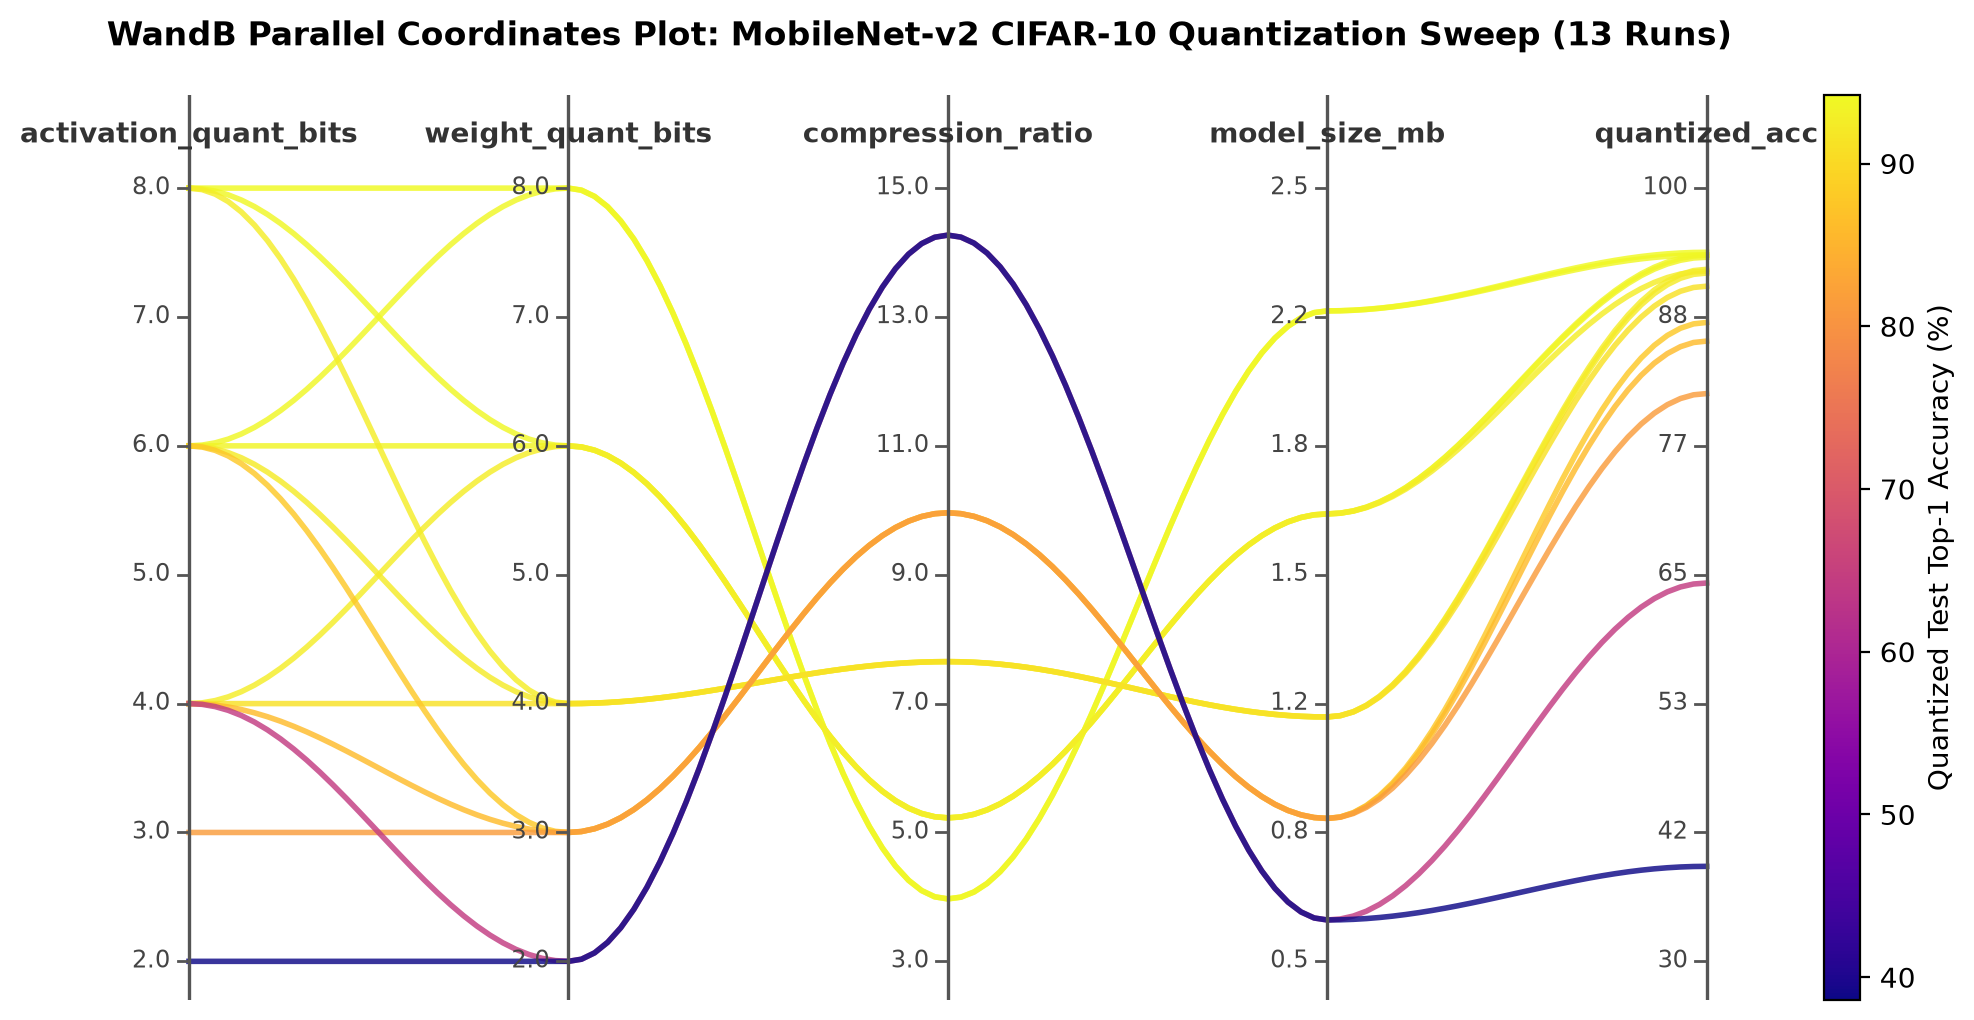
\includegraphics[width=0.98\textwidth]{../results/parallel_coordinates.png}
\caption{WandB Parallel Coordinates chart across all 13 compression runs (\texttt{sweep.py}), plotting \texttt{activation\_quant\_bits}, \texttt{weight\_quant\_bits}, \texttt{compression\_ratio}, \texttt{model\_size\_mb}, and \texttt{quantized\_acc}.}
\label{fig:parallel_coords}
\end{figure}

\begin{figure}[ht!]
\centering
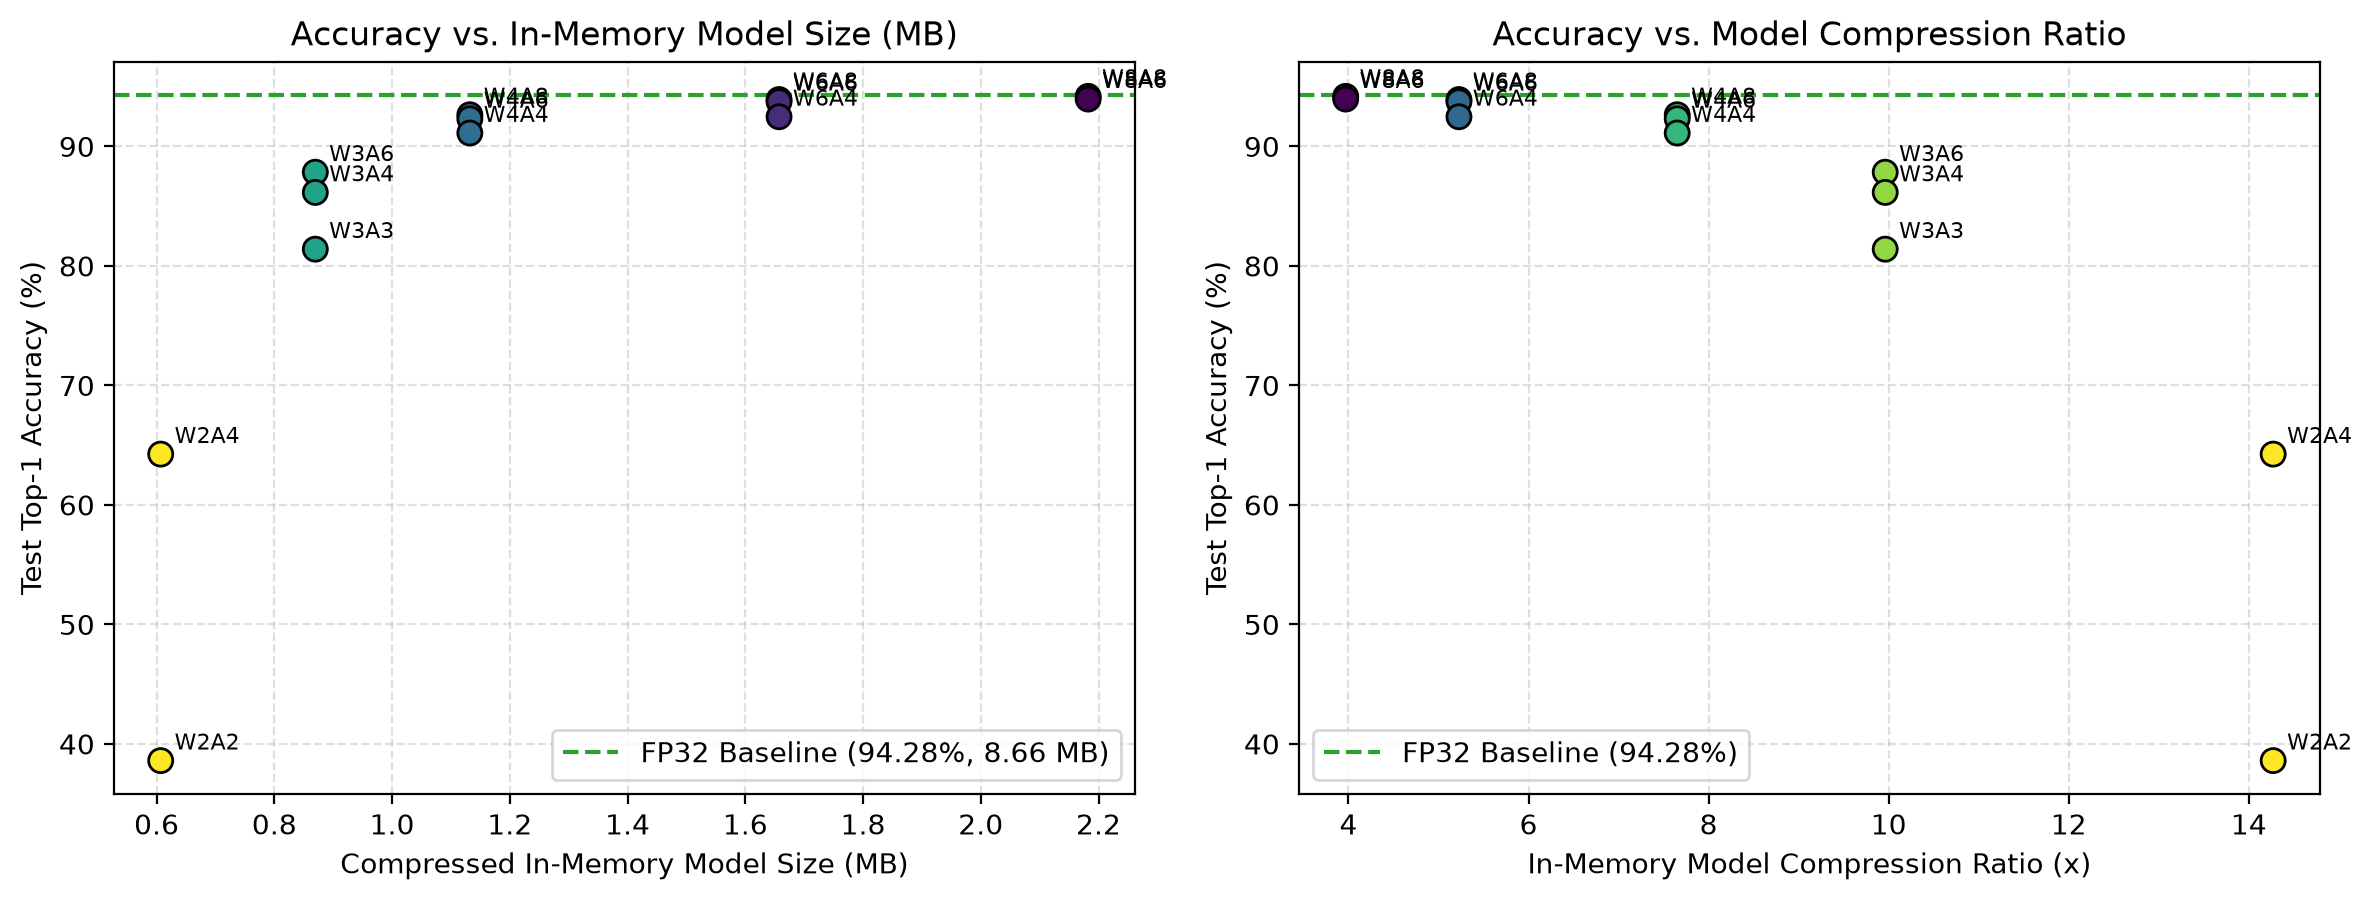
\includegraphics[width=0.98\textwidth]{../results/compression_pareto.png}
\caption{Pareto frontier of Test Top-1 Accuracy vs.\ Compressed In-Memory Model Size (MB) and Model Compression Ratio across the 13 bit-width configurations.}
\label{fig:pareto}
\end{figure}

% ============================================================================
\section*{Question 4. Compression Analysis}
% ============================================================================

\subsection*{(a) Compression Ratio of the Weights (In-Memory)}
Uncompressed Conv2d and Linear weights occupy $2,202,570 \times 4\text{ B} = \mathbf{8,810,280\text{ Bytes}}$ (\textbf{8.4021 MB}). Including per-channel FP16 scales ($34,132\text{ B}$) and \texttt{uint8} zero-points ($17,066\text{ B}$), the weight compression ratio is:
\[
\text{CR}_{\text{weights}}(b_w) = \frac{8,810,280}{\sum_{l=1}^{53} \lceil N_l b_w / 8 \rceil + 34,132 + 17,066} =
\begin{cases}
\mathbf{3.91\times} & (b_w = 8\text{ bits}, \;\text{Packed } W = 2.1005\text{ MB}) \\
\mathbf{5.17\times} & (b_w = 6\text{ bits}, \;\text{Packed } W = 1.5754\text{ MB}) \\
\mathbf{7.64\times} & (b_w = 4\text{ bits}, \;\text{Packed } W = 1.0503\text{ MB}) \\
\mathbf{10.04\times} & (b_w = 3\text{ bits}, \;\text{Packed } W = 0.7877\text{ MB}) \\
\mathbf{14.64\times} & (b_w = 2\text{ bits}, \;\text{Packed } W = 0.5251\text{ MB})
\end{cases}
\]
Because BatchNorm folding additionally eliminates $272,896\text{ Bytes}$ (266.50 KB) of BatchNorm parameters and running buffers, the \textbf{overall in-memory model compression ratio} reaches \textbf{3.97$\times$} (W8), \textbf{5.23$\times$} (W6), \textbf{7.65$\times$} (W4), \textbf{9.96$\times$} (W3), and \textbf{14.27$\times$} (W2).

\subsection*{(b) Compression Ratio of the Activations \& Measurement Methodology}
\textbf{Measurement Methodology (\texttt{compression/memory\_profiler.py}):}
We register PyTorch forward hooks (\texttt{register\_forward\_hook}) on all 53 quantized layers during a forward pass of a $32\times 32$ CIFAR-10 image ($B=1$) and measure two distinct metrics:
\begin{enumerate}\setlength\itemsep{1pt}
    \item \textbf{Cumulative Layer Activation Memory:} Sum of all 53 input activation tensors across the network: $\sum_{l=1}^{53} \text{numel}(X_l) = 1,623,808$ elements = \textbf{6,343.00 KB (6.194 MB)} in FP32.
    \item \textbf{Peak Live Working-Set Activation Memory:} Maximum simultaneous memory required by any single layer's input + output feature maps, which occurs at \texttt{features.3} ($3\times 3$ depthwise conv on $144 \times 32 \times 32$): $147,456 + 147,456 = 294,912$ elements = \textbf{1,152.00 KB (1.125 MB)} in FP32.
\end{enumerate}
Including the 3-byte per-tensor scale/zero-point metadata per layer ($53 \times 3 = 159\text{ Bytes}$), the measured activation compression ratios are:
\begin{itemize}\setlength\itemsep{1pt}
    \item \textbf{8-bit Activations (A8):} $6,343.00\text{ KB} \to 1,585.91\text{ KB}$ (\textbf{4.00$\times$ cumulative}, \textbf{4.00$\times$ peak live}: $1,152.00\text{ KB} \to 288.01\text{ KB}$).
    \item \textbf{6-bit Activations (A6):} $6,343.00\text{ KB} \to 1,189.47\text{ KB}$ (\textbf{5.33$\times$ cumulative}, \textbf{5.33$\times$ peak live}: $1,152.00\text{ KB} \to 216.01\text{ KB}$).
    \item \textbf{4-bit Activations (A4):} $6,343.00\text{ KB} \to 793.03\text{ KB}$ (\textbf{8.00$\times$ cumulative}, \textbf{8.00$\times$ peak live}: $1,152.00\text{ KB} \to 144.01\text{ KB}$).
    \item \textbf{3-bit Activations (A3):} $6,343.00\text{ KB} \to 594.81\text{ KB}$ (\textbf{10.66$\times$ cumulative}, \textbf{10.67$\times$ peak live}: $1,152.00\text{ KB} \to 108.01\text{ KB}$).
    \item \textbf{2-bit Activations (A2):} $6,343.00\text{ KB} \to 396.59\text{ KB}$ (\textbf{15.99$\times$ cumulative}, \textbf{16.00$\times$ peak live}: $1,152.00\text{ KB} \to 72.01\text{ KB}$).
\end{itemize}

\subsection*{(v) Final Approximated Model Size (MB) After Compression}
\begin{itemize}\setlength\itemsep{1pt}
    \item \textbf{Lossless-Grade Setting (\texttt{W8A8}):} \textbf{2.1824 MB} (94.19\% accuracy, 3.97$\times$ smaller than 8.6624 MB baseline).
    \item \textbf{High-Accuracy Pareto Setting (\texttt{W4A4}):} \textbf{1.1321 MB} (91.12\% accuracy, \textbf{7.65$\times$} model compression, \textbf{8.00$\times$} activation compression).
    \item \textbf{Sub-Megabyte Setting (\texttt{W3A4}):} \textbf{0.8696 MB} (86.15\% accuracy, \textbf{9.96$\times$} model compression).
    \item \textbf{Extreme Compression Setting (\texttt{W2A2}):} \textbf{0.6070 MB} (\textbf{14.27$\times$} model compression).
\end{itemize}

% ============================================================================
\section*{Question 5. Reproducibility \& Repository (10 Points)}
% ============================================================================

\begin{itemize}\setlength\itemsep{3pt}
    \item \textbf{(a) Modular Codebase Architecture (4 pts):} Separated into \texttt{data.py} (CIFAR-10 transforms \& Cutout), \texttt{models/mobilenetv2.py} ($32\times 32$ MobileNet-v2), \texttt{compression/bitpack.py} (sub-byte \texttt{uint8} bit-stream packing), \texttt{compression/quantizer.py} (BatchNorm folding, \texttt{QuantizedConv2d}, \texttt{QuantizedLinear}, \texttt{ActivationQuantizer}), \texttt{compression/memory\_profiler.py} (RAM/VRAM \& hook profiler), \texttt{train.py}, \texttt{test.py}, and \texttt{sweep.py}.
    \item \textbf{(b) Exact Reproduction Commands \& Deterministic Seed (4 pts):} All runs fix \texttt{seed=42} across \texttt{random}, \texttt{numpy}, \texttt{torch}, and \texttt{cudnn.deterministic=True}:
\begin{lstlisting}[language=bash]
# 1. Train Baseline MobileNet-v2 on CIFAR-10 (94.28% Top-1 Accuracy)
python train.py --epochs 200 --batch_size 128 --lr 0.05 --seed 42

# 2. Evaluate Custom Compression (Template CLI Compatible)
python test.py --weight_quant_bits 8 --activation_quant_bits 8
python test.py --weight_quant_bits 4 --activation_quant_bits 4

# 3. Run 13-Configuration Compression Sweep & Generate Plots
python sweep.py --checkpoint ./checkpoints/mobilenetv2_cifar10_best.pth --use_wandb
python generate_plots.py
\end{lstlisting}
    \item \textbf{(c) GitHub Repository Link (2 pts):} \url{https://github.com/cs25m513/CS6886W-Assignment2-MobileNetV2}
\end{itemize}

\end{document}
